% $Id: chapter3.tex 1790 2010-09-28 16:46:40Z jabriffa $

\chapter{System Analysis}

\section{Feasibility and System Limitations}
The project was designed as a demonstration to show how a let-alone, but personalized social news aggregator would work. The system flagship features of competing systems, all while mitigating issues such as the need of moderators to manage common issues such as vote-rigging or out-of-place content that disrupt the culture of the website.

Even though the system achieves the project's scope, that is not to say the system has reached its potential. There are many solutions that could perhaps increase the project's quality. For example, in order to improve sorting over time, the user could set their original interests but, over time a NN could monitor the user's actions and alter their interests judging from the way they interact with posts, such as time spent reading on a post that had other interests that the user did not initially mark as desirable. That way, the AI would create some hidden ranking that would sort the posts by that rank. It would not come with complications; nevertheless, building and running such a network would require not only immense dedicated computing power but also, periodic monitoring and safety regulation.

Changing the project's objectives and looking into lesser-known existing websites and their solutions in the literature review could likely provide more information on how these other systems handle sorting and what intricacies are involved when sorting information. Making the project more complex would defeat the goal of the project and could result in an overwhelming experience for the user. Moreover, in order for this project to yield meaningful results and an enjoyable experience results, responsiveness is key, which by overloading the system could result in the lack of those aspects.

\section{User Experience}
In order to create a user-friendly interface and experience, the front end of the website was made entirely in Boostrap. Bootstrap is a free and open-source CSS framework directed at responsive, mobile-first front-end web development. It contains CSS- and (optionally) JavaScript-based design templates for typography, forms, buttons, navigation, and other interface components

\cite{wikipediacontributors_2019_bootstrap}. This allowed me to make a very clean and friendly user interface.

Bootstrap uses default colours for different types of importance as visible:

\begin{figure}[!h]
  \centering
	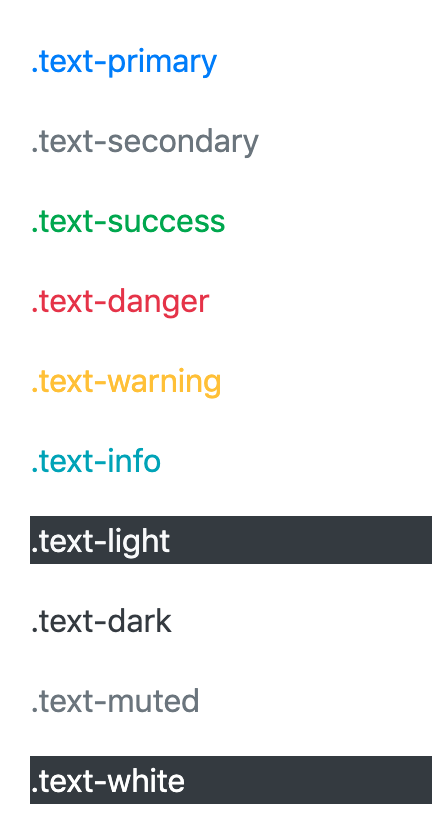
\includegraphics[scale=0.5]{Figures/bootstrap_colours}
\caption{}
\end{figure}

\section{Problems and Proposed Solutions}

\section{Interview \& Survey}
